\chapter{Risultati}

\section{Approccio}
L'obiettivo del sistema proposto è quello di lavorare near real-time, vincolato sia dai tempi di risposta della API, sia dallo use case presentato nel capitolo precedente. Al momento, si vuole validare la presenza dei DPI indossati da un lavoratore in una zona limitrofa al macchinario. % e periodicamente verificare che la condizione sia rispettata. 
Inoltre, in Rekognition, le richieste di analisi dei frame, vengono soddisfatte in tempi superiori al decimo di secondo, il che rende la prevenzione degli incidenti ancora difficile da realizzare. L'approccio utilizzato, come visto nell'implementazione del sistema, è quello di ricevere i dati via streaming, iniziando l'analisi il prima possibile, sfruttando sia il parallelismo nel preprocessing, che la reazione granulare agli eventi nell'applicazione big data. I risultati seguono in maniera coerente questa logica, per cui il focus in questa sezione è più orientato al tempo globale di risposta, ed alla soglia di frame processati correttamente. Questa scelta è motivata da diverse necessità, sotto l'ipotesi che il modello di base abbia delle buone prestazioni, ma che in certe condizioni non performi correttamente. In primo luogo si vuole ottenere robustezza per le detection errate, effetto della generazione di falsi positivi e negativi. Infatti, come visto anche nei lavori correlati, è possibile che un dato oggetto non venga trovato, oppure che la predizione della classe sia errata. In secondo luogo, non avrebbe senso spegnere e riaccendere il macchinario a causa delle fluttuazioni nei rilevamenti, rendendo di fatto l'utilità del sistema poco significativa. Infine, avere un campione di un intervallo di frame permette di compensare potenziali rumori durante la registrazione, come movimenti rapidi, variazioni di angolazione ed occlusioni temporanee. 



\section{Test case e analisi}
%documentazione amazon
%La documentazione Amazon non fornisce dettagli riguardo le prestazioni del modello, sia per le rilevazioni generiche che per il caso speciale in esame. Nel primo caso, tuttavia, esiste un confronto di Rekognition con altri modelli State-of-the-art(Sota), mostrato in un articolo di Roboflow.

%roboflow
%Per il caso specifico dei DPI, è stata eseguita una analisi preliminare del modello, in modo tale da avere, seppur in maniera limitata, un confronto con gli altri lavori svolti in questo campo. Per eseguire la valutazione, è stato scelto il dataset CHV, dal quale sono state estratte le metriche per il rilevamento dei caschi protettivi. %vedi se riesci ad aggiungere anche le persone.
%dataset
%ap per i caschi, iou 0.5 e 0.7 ed infine map per le iou
%grafico a pallini per tempi di riposta di rekognition e del sistema con tutti i campioni
I test sono stati eseguiti con oggetto solo la rilevazione del casco protettivo, generando un campione che prevede i seguenti parametri:

\begin{itemize}
	\item \textbf{tags}: indica il totale dei tag associati alle persone interne all'area di sicurezza; può non esprimere realmente il numero di lavoratori, in quanto non tutti potrebbero avere il tag aziendale.
	\item \textbf{people}: è il numero di individui effettivamente presenti nell'area di sicurezza. 
	\item \textbf{equipment}: definisce se il lavoratore indossa il casco, indipendemente dall'esito dell'analisi.
	\item \textbf{machine state}: è il valore della macchina all'inizio del test; in questa valutazione è sempre stato impostato come acceso.
%	\item \textbf{ppe percentage}: si tratta della percentuale di frame in cui i caschi sono stati rilevati.
%	\item \textbf{matching people percentage}: è la frazione di immagini in cui il numero di persone rilevate dal modello di visione artificiale corrisponde al numero di persone identificate dai tag.
	\item \textbf{expected result}: è l'azione attesa a valle dell'analisi, quindi generazione dell'allarme. 
	
\end{itemize}	

I test case sono mostrati in Tabella \ref{tab:test-cases} ciascuno di essi è stato lanciato 10 volte. Questo metodo è stato applicato iterativamente in giornate e luoghi differenti, tenendo così conto della variabilità dell'ambiente e della luminosità.  


\begin{table}[htbp]
\centering
\begin{tabular}{|c|c|c|c|c|c|}
\toprule
\textbf{tags} & \textbf{people} & \textbf{eqipment} & \textbf{machine state} & \textbf{Rexpected} \\ \midrule

 0 & 1 & TRUE & TRUE & ALARM  \\ \midrule
 1 & 1 & FALSE & TRUE & ALARM     \\ \midrule
 0 & 1 & FALSE & TRUE & ALARM    \\ \midrule
 2 & 2 & TRUE;FALSE & TRUE & ALARM    \\ \midrule
 1 & 2 & TRUE;FALSE & TRUE & ALARM    \\ \midrule
\end{tabular}
\caption{Test case.}
\label{tab:test-cases}
\end{table}

Il sistema si è comportato correttamente in quasi tutte le prove. Nel primo scenario ha rilevato il dispositivo di sicurezza in tutti i frame per ciascun test. In un solo caso il modello è riuscito a vedere il casco nell'80\% dei frame, ma comunque la detection globalmente è andata a buon fine, perché la soglia di rilevazione complessiva è stata impostata al 70\%. Per tutte le restanti prove invece la percentuale di frame ottenuta è stata nulla, in quanto il dispositivo non era indossato almeno da una persona. Per quanto riguarda il numero di persone contate, i risultati sono stati quelli attesi: il modello è sempre stato in grado di effettuare correttamente il conteggio ed il matching è andato a buon fine per tutto il gruppo di frame in ciascuna analisi. Di conseguenza, le regole per l'attivazione dell'allarme si sono sempre verificate.

Per quanto riguarda i tempi di risposta, il sistema rientra nei parametri near real-time, in quanto non ha un framerate superiore a 5fps, considerata la soglia minima per essere classificato come real-time puro. Tipicamente, in questo dominio, viene considerato near real-time un tempo di processamento nell'ordine dei secondi o dei minuti. Il delay tra la prima richiesta a Rekognition e la risposta per l'ultimo frame analizzato è di circa 850ms. L'applicazione big data invece impiega mediamente 550ms per ricevere gli input ed eventualmente inviare l'allarme. Quelle appena viste sono metriche di più basso livello, nell'ottica di quantificare l'impatto di ciascun servizio Amazon sul sistema. La misura più importante, tuttavia, resta la latenza totale dalla generazione dell'evento tramite i sensori, fino al ritorno dell'analisi nell'area di lavoro. La media ottenuta dai campioni generati in fase di test è stata di 2,56 secondi con una deviazione standard di 0,374.

\begin{figure}[htbp]
    \centering
    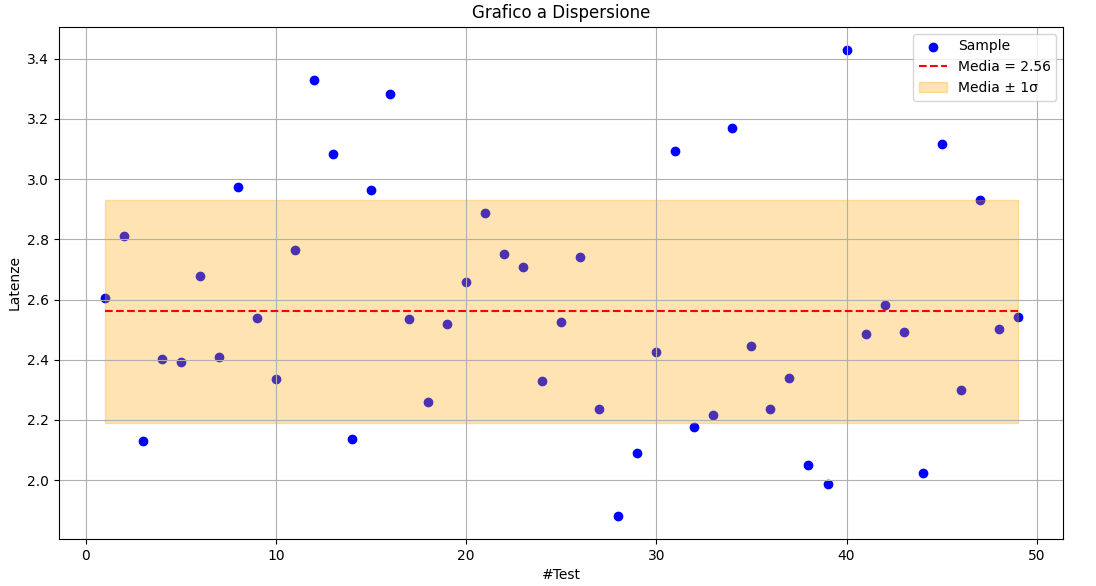
\includegraphics[width=0.9\textwidth]{figures/system-latency.png}
    \caption{Latenza totale del sistema.} 
    \label{fig:system-latency}
\end{figure}

\section{Limitazioni}











%il sistema è stato pensato in questo modo anche per adattamento 
%incompatibilità con le classi di confronto; dataset malformati o non disponibili;
I test sono stati eseguiti con le immagini acquisite dalle telecamere, ma non sono state svolte in un ambiente industriale, come nel caso dei related works. Inoltre le metriche considerate non sono rapportabili, quindi servirebbero ulteriori indagini in questa direzione. Si tratterebbe comunque di una valutazione imparziale in quanto i modelli di riferimento sono stati installati direttamente nell'area industriale e non si trovano sul cloud. In primo luogo è necessario generare un modello installabile sull'edge, ma Amazon non offre questa possibilità con il servizio Rekognition, pensato per soluzioni che non necessitano allenamenti o installazioni, come visto nella sezione dei servizi AWS. Per potersi allineare ai lavori citati occorre quindi scegliere un'altra opzione che integra edge e cloud contemporaneamente, cioé SageMaker. Sarebbe possibile in questo caso sfruttare l'infrastruttura AWS per semplificare la gestione del ciclo di vita di un modello custom, generato su un dataset ad hoc. Si dovrebbe seguire lo stesso approccio per avere le migliori prestazioni possibili: il modello deve adattarsi ad un ambiente specifico e quindi necessita della generazione di immagini storiche dalla fabbrica e di un processo di etichettatura. Se si dovesse sviluppare l'applicazione near real-time con il deploy sul cloud, le prestazioni sarebbero migliori già in termini di latenza, perché non si sfrutterebbe la API di un servizio gestito, pensato per essere utilizzato in larga scala da un numero indefinito di utenti.     

Un'altra limitazione di questa analisi riguarda l'ambiente di test, che al momento non è automatizzato. Si deve infatti eseguire manualmente degli script e modificare i parametri in base al test case. Per eseguire i test non sono stati utilizzati dei dati provenienti dai sensori, ma viene simulato il JSON che si otterrebbe alla generazione dell'evento per lo scenario specifico. L'analisi dei frame nei test avviene tramite live streaming, ma sarebbe più opportuno definire come source un insieme standard di video storici in modo da rendere i test facilmente ripetibili. L'automatizzazione dell'insieme di test invece sarebbe attuabile tramite degli orchestratori. Nell'ecosistema AWS esiste un servizo per questo tipo di scenario, le Step Functions. Affinché questo workflow venga implementato ogni volta che ci sono modifiche al sistema occorrerebbe integrare il tutto all'interno di una pipeline CI/CD, dove ad ogni commit si invoca l'orchestratore per eseguire tutti i test necessari. Questo meccanismo inoltre non si limiterebbe solo ai test, ma anche al build del codice, al deploy dell'infrastruttura ed infine al monitoraggio. AWS offre un servizio integrato apposito per le pratiche di devops chiamato CodePipeline. Un drawback relativo alla valutazione del sistema, correlato in parte all'impossibilità di esecuzione in un ambiente industriale, è il fatto di essersi limitato a sole due telecamere. Idealmente, bisognerebbe testare funzionalità e prestazioni su un set maggiore di dispositivi, in modo tale da verificare la risposta del sistema in scala. Sarebbe inoltre utile testare in maniera coerente anche l'integrazione con i sensori, che sebbene la generazione simulata degli eventi renda i test attendibili, con buona probabilità non tiene conto di eventuali problematiche che si aggiungono in un caso reale. Ad esempio dovrebbero essere verificati eventuali disconessioni e problemi di sincronizzazione. 
Infine, un'ultima limitazione di questa analisi riguarda la potenza del gateway: la macchina server utilizzata non ha la potenza di calcolo necessaria per supportare l'interazione con un numero elevato di dispositivi, soprattutto per quel che riguarda l'inoltro dello stream. Infatti durante la valutazione, anche con un ambiente minimale, si è notato un grosso overhead causato soprattutto dai tempi di codifica e decodifica dei flussi video provenienti dai source RTSP.  

\section{Lavori futuri}

%integrazione con robot
Eventuali estensioni del sistema dovrebbero in una prima fase rispondere alle limitazioni appena citate, di cui sono già state proposte alcune soluzioni. Successivamente occore operare in altre aree per il completamento del prototipo, come l'integrazione con i robot. Ciò avviene tramite la generazione di un container apposito, simile a quanto fatto per il gateway, ma direttamente sui dispositivi. La macchina virtuale al suo interno conterrà una immagine basata su un sistema operativo real time per la robotica, ad esempio ROS, sopra il quale dovrà essere presente una installazione Greengrass, per facilitare l'integrazione con il cloud. In questo modo si ottengono tutti i vantaggi del runtime, che nel caso di applicazioni legate alla robotica diventano vitali. La gestione remota della telemetria e gli update per sistemi di questo tipo creano molti problemi ai produttori, sia in termini di affidabilità che di tempo. Realizzare delle soluzioni apposite infatti richiede un effort notevole alle aziende specializzate in questo campo. L'utilizzo di un container, inoltre, offre anche il vantaggio di non interferire con l'ambiente dell'host: un eventuale crash di un'applicazione in questo scenario potrebbe compromettere il funzionamento del robot. L'integrazione con ROS, permette di gestire in maniera molto semplice la comunicazione interna con il robot, in quanto l'invio dei comandi o la comunicazione locale tra varie macchine è coordinata da meccanismi publish/subscribe. Per l'attivazione/disattivazione della macchina bisogna pubblicare l'esito dell'analisi su un topic MQTT di AWS IoT core, al quale i robot interessati saranno iscritti. A questo punto, un componente Greengrass installato sulla macchina si occuperà di processare il messaggio. L'ultima operazione è quella di inoltro del risultato su un topic ROS, che in base alla condizione, eseguirà il comando di accensione o spegnimento.

%rule dinamiche e monitoraggio
A livello di processamento big data, invece, Apache Flink offre dei meccanismi più sofisticati nella gestione delle regole. Il sistema attuale, ad esempio, non si adatta alla variabilità delle condizioni nell'ambiente di lavoro. Potrebbero esserci cambiamenti della luminosità, oppure altri effetti che impattano sull'analisi delle immagini, di conseguenza sulle percentuali di frame con rilevazioni corrette. A quel punto, il sistema, dovrebbe essere in grado di aggiornare le soglie tramite comandi remoti, provenienti dai sistemi di monitoraggio, invece di un redeploy con le nuove regole. Il set delle possibili azioni dovrebbe essere salvato in un database che si adatta facilmente a questo tipo di applicazione, come DynamoDB. 

Per quel che riguarda il tracciamento globale edge-cloud, allo stato attuale i flussi di log sono molto semplici e coinvolgono soltanto il preprocessing, ma dovrebbero essere estesi anche a quelli prodotti dall'applicazione big data e dal gateway. Il tutto, grazie a CloudWatch, verrebbe gestito in maniera centralizzata e, con riferimento ai device in fabbrica, anche remota. 

%salvataggio di eventi
Infine, l'ultimo sviluppo fondamentale, al di fuori della main business logic, sarebbe quello di generare delle statistiche sul corretto utilizzo dei dispositivi di sicurezza, salvando le informazioni più importanti associate agli eventi di interesse, mostrate su una eventuale interfaccia utente.